% Part-Set Fusion V7 — parameter budget figure (research-paper style)
% Build:  pdflatex v7_parameter_budget.tex
% Counts measured directly from the built model (designs/skeleton_silhouette_partset_v7):
%   TOTAL 6,203,429
%   decoder (train only)      3,625,914  58.5%
%   Bi-GRU temporal branch    1,040,737  16.8%   (temporal_cnn + temporal_rnn + attention)
%   embedding head              755,968  12.2%
%   shared trunk                489,600   7.9%
%   part branch                 126,720   2.0%   (part_motion + part_fc)
%   projector + classifier      117,706   1.9%
%   stems (sil + skel)           38,400   0.6%
%   spatial gate                  8,384   0.1%
% Inference path = total - decoder - classifier - projector = 2,459,809 (2.46 M)
\documentclass[tikz, border=12pt]{standalone}
\usepackage[T1]{fontenc}
\renewcommand{\familydefault}{\sfdefault}
\usetikzlibrary{positioning, calc}

\definecolor{decbrown}{RGB}{181,159,140}
\definecolor{grupurple}{RGB}{146,118,190}
\definecolor{embgray}{RGB}{96,109,122}
\definecolor{trunkblue}{RGB}{78,121,167}
\definecolor{partgreen}{RGB}{89,161,105}
\definecolor{headlight}{RGB}{186,196,204}
\definecolor{stemblue}{RGB}{158,193,225}
\definecolor{gateorange}{RGB}{237,173,79}
\definecolor{inkdark}{RGB}{45,45,45}
\definecolor{titlebrown}{RGB}{176,88,38}

\tikzset{
  seg/.style={draw=white, line width=0.8pt},
  seglbl/.style={font=\small\bfseries, text=white},
  legsq/.style={draw=#1!60!black, fill=#1, minimum size=3.2mm, inner sep=0pt},
  leglbl/.style={font=\scriptsize, text=inkdark},
}

% bar length in cm per 100%
\newcommand{\BARLEN}{24.0}
\newcommand{\BARH}{1.35}

\begin{document}
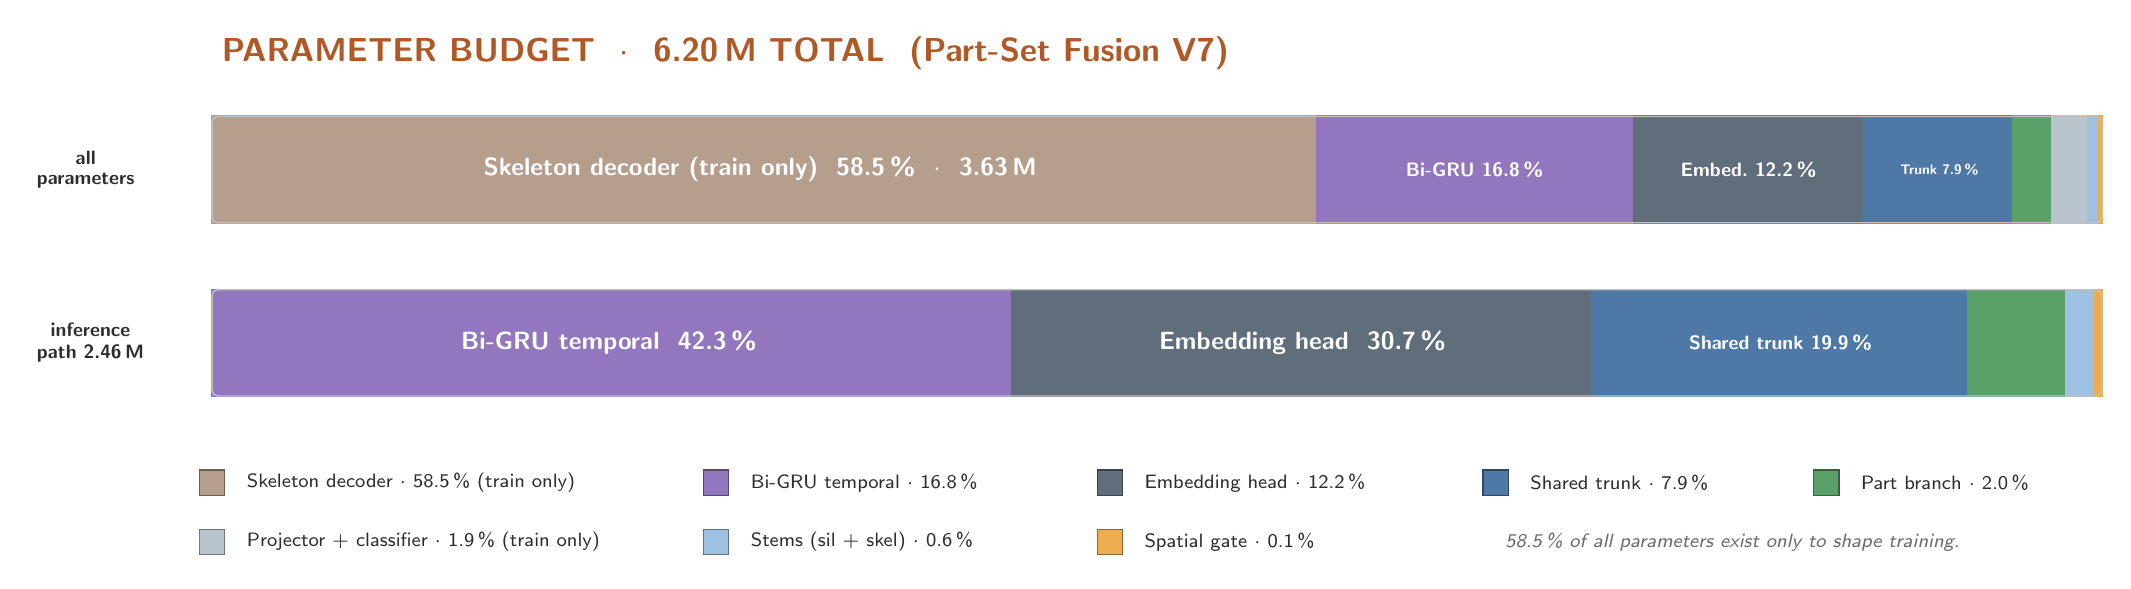
\begin{tikzpicture}[x=1cm, y=1cm]

% ============================================================ title
\node[anchor=west, font=\large\bfseries, text=titlebrown] at (0, 4.15)
  {PARAMETER BUDGET\ \ $\cdot$\ \ 6.20\,M TOTAL\ \ (Part-Set Fusion V7)};

% ============================================================ bar 1: total
% cumulative fractions: 58.45, 16.78, 12.19, 7.89, 2.04, 1.90, 0.62, 0.14
\begin{scope}[shift={(0, 2.0)}]
  \fill[seg, decbrown]   (0.0000*\BARLEN, 0) rectangle (0.5845*\BARLEN, \BARH);
  \fill[seg, grupurple]  (0.5845*\BARLEN, 0) rectangle (0.7523*\BARLEN, \BARH);
  \fill[seg, embgray]    (0.7523*\BARLEN, 0) rectangle (0.8742*\BARLEN, \BARH);
  \fill[seg, trunkblue]  (0.8742*\BARLEN, 0) rectangle (0.9531*\BARLEN, \BARH);
  \fill[seg, partgreen]  (0.9531*\BARLEN, 0) rectangle (0.9735*\BARLEN, \BARH);
  \fill[seg, headlight]  (0.9735*\BARLEN, 0) rectangle (0.9925*\BARLEN, \BARH);
  \fill[seg, stemblue]   (0.9925*\BARLEN, 0) rectangle (0.9987*\BARLEN, \BARH);
  \fill[seg, gateorange] (0.9987*\BARLEN, 0) rectangle (1.0000*\BARLEN, \BARH);
  \draw[inkdark!30, line width=0.5pt, rounded corners=2pt] (0,0) rectangle (\BARLEN, \BARH);

  \node[seglbl] at (0.29*\BARLEN, 0.5*\BARH) {Skeleton decoder (train only)\ \ 58.5\,\%\ \ $\cdot$\ \ 3.63\,M};
  \node[seglbl, font=\scriptsize\bfseries] at (0.668*\BARLEN, 0.5*\BARH) {Bi-GRU\ 16.8\,\%};
  \node[seglbl, font=\scriptsize\bfseries] at (0.813*\BARLEN, 0.5*\BARH) {Embed.\ 12.2\,\%};
  \node[seglbl, font=\tiny\bfseries] at (0.914*\BARLEN, 0.5*\BARH) {Trunk 7.9\,\%};
  \node[font=\scriptsize\bfseries, text=inkdark, anchor=west] at (-2.35, 0.5*\BARH) {\shortstack{all\\parameters}};
\end{scope}

% ============================================================ bar 2: inference path
% inference path 2,459,809: trunk 19.90, GRU 42.31, embedding 30.73, part 5.15, stems 1.56, gate 0.34
\begin{scope}[shift={(0, -0.2)}]
  \fill[seg, grupurple]  (0.0000*\BARLEN, 0) rectangle (0.4231*\BARLEN, \BARH);
  \fill[seg, embgray]    (0.4231*\BARLEN, 0) rectangle (0.7304*\BARLEN, \BARH);
  \fill[seg, trunkblue]  (0.7304*\BARLEN, 0) rectangle (0.9294*\BARLEN, \BARH);
  \fill[seg, partgreen]  (0.9294*\BARLEN, 0) rectangle (0.9810*\BARLEN, \BARH);
  \fill[seg, stemblue]   (0.9810*\BARLEN, 0) rectangle (0.9966*\BARLEN, \BARH);
  \fill[seg, gateorange] (0.9966*\BARLEN, 0) rectangle (1.0000*\BARLEN, \BARH);
  \draw[inkdark!30, line width=0.5pt, rounded corners=2pt] (0,0) rectangle (\BARLEN, \BARH);

  \node[seglbl] at (0.21*\BARLEN, 0.5*\BARH) {Bi-GRU temporal\ \ 42.3\,\%};
  \node[seglbl] at (0.577*\BARLEN, 0.5*\BARH) {Embedding head\ \ 30.7\,\%};
  \node[seglbl, font=\scriptsize\bfseries] at (0.83*\BARLEN, 0.5*\BARH) {Shared trunk\ 19.9\,\%};
  \node[font=\scriptsize\bfseries, text=inkdark, anchor=west] at (-2.35, 0.5*\BARH) {\shortstack{inference\\path\ 2.46\,M}};
\end{scope}

% ============================================================ legend
\begin{scope}[shift={(0, -1.3)}]
  \node[legsq=decbrown]   (g1) at (0.0, 0) {};
  \node[leglbl, right=1.5mm of g1] {Skeleton decoder $\cdot$ 58.5\,\% (train only)};
  \node[legsq=grupurple]  (g2) at (6.4, 0) {};
  \node[leglbl, right=1.5mm of g2] {Bi-GRU temporal $\cdot$ 16.8\,\%};
  \node[legsq=embgray]    (g3) at (11.4, 0) {};
  \node[leglbl, right=1.5mm of g3] {Embedding head $\cdot$ 12.2\,\%};
  \node[legsq=trunkblue]  (g4) at (16.3, 0) {};
  \node[leglbl, right=1.5mm of g4] {Shared trunk $\cdot$ 7.9\,\%};
  \node[legsq=partgreen]  (g5) at (20.5, 0) {};
  \node[leglbl, right=1.5mm of g5] {Part branch $\cdot$ 2.0\,\%};

  \node[legsq=headlight]  (g6) at (0.0, -0.75) {};
  \node[leglbl, right=1.5mm of g6] {Projector $+$ classifier $\cdot$ 1.9\,\% (train only)};
  \node[legsq=stemblue]   (g7) at (6.4, -0.75) {};
  \node[leglbl, right=1.5mm of g7] {Stems (sil $+$ skel) $\cdot$ 0.6\,\%};
  \node[legsq=gateorange] (g8) at (11.4, -0.75) {};
  \node[leglbl, right=1.5mm of g8] {Spatial gate $\cdot$ 0.1\,\%};
  \node[leglbl, text=inkdark!70, font=\scriptsize\itshape, anchor=west] at (16.3, -0.75)
    {58.5\,\% of all parameters exist only to shape training.};
\end{scope}

\end{tikzpicture}
\end{document}
